% Options for packages loaded elsewhere
\PassOptionsToPackage{unicode}{hyperref}
\PassOptionsToPackage{hyphens}{url}
%
\documentclass[
]{article}
\usepackage{amsmath,amssymb}
\usepackage{iftex}
\ifPDFTeX
  \usepackage[T1]{fontenc}
  \usepackage[utf8]{inputenc}
  \usepackage{textcomp} % provide euro and other symbols
\else % if luatex or xetex
  \usepackage{unicode-math} % this also loads fontspec
  \defaultfontfeatures{Scale=MatchLowercase}
  \defaultfontfeatures[\rmfamily]{Ligatures=TeX,Scale=1}
\fi
\usepackage{lmodern}
\ifPDFTeX\else
  % xetex/luatex font selection
\fi
% Use upquote if available, for straight quotes in verbatim environments
\IfFileExists{upquote.sty}{\usepackage{upquote}}{}
\IfFileExists{microtype.sty}{% use microtype if available
  \usepackage[]{microtype}
  \UseMicrotypeSet[protrusion]{basicmath} % disable protrusion for tt fonts
}{}
\makeatletter
\@ifundefined{KOMAClassName}{% if non-KOMA class
  \IfFileExists{parskip.sty}{%
    \usepackage{parskip}
  }{% else
    \setlength{\parindent}{0pt}
    \setlength{\parskip}{6pt plus 2pt minus 1pt}}
}{% if KOMA class
  \KOMAoptions{parskip=half}}
\makeatother
\usepackage{xcolor}
\usepackage[margin=1in]{geometry}
\usepackage{graphicx}
\makeatletter
\def\maxwidth{\ifdim\Gin@nat@width>\linewidth\linewidth\else\Gin@nat@width\fi}
\def\maxheight{\ifdim\Gin@nat@height>\textheight\textheight\else\Gin@nat@height\fi}
\makeatother
% Scale images if necessary, so that they will not overflow the page
% margins by default, and it is still possible to overwrite the defaults
% using explicit options in \includegraphics[width, height, ...]{}
\setkeys{Gin}{width=\maxwidth,height=\maxheight,keepaspectratio}
% Set default figure placement to htbp
\makeatletter
\def\fps@figure{htbp}
\makeatother
\setlength{\emergencystretch}{3em} % prevent overfull lines
\providecommand{\tightlist}{%
  \setlength{\itemsep}{0pt}\setlength{\parskip}{0pt}}
\setcounter{secnumdepth}{5}
\usepackage{booktabs,longtable,dcolumn} \usepackage{multirow,array} \usepackage{wrapfig,float} \floatplacement{figure}{H}
\ifLuaTeX
  \usepackage{selnolig}  % disable illegal ligatures
\fi
\IfFileExists{bookmark.sty}{\usepackage{bookmark}}{\usepackage{hyperref}}
\IfFileExists{xurl.sty}{\usepackage{xurl}}{} % add URL line breaks if available
\urlstyle{same}
\hypersetup{
  pdftitle={QuickPay Delay Rate -- All Defense Projects},
  hidelinks,
  pdfcreator={LaTeX via pandoc}}

\title{QuickPay Delay Rate -- All Defense Projects}
\author{}
\date{\vspace{-2.5em}2024-06-18}

\begin{document}
\maketitle

\hypertarget{quickpay-expanded-sample}{%
\section{QuickPay Expanded Sample}\label{quickpay-expanded-sample}}

\begin{itemize}
\tightlist
\item
  Consider ALL defense projects that started b/w FY 2010 and FY 2012
\item
  Consider ALL action types
\item
  Treat is N/A for Small Disadvantaged Business (i.e., they are
  excluded)
\item
  Restrict to June 30, 2012 -- QP expanded to all projects after that
\end{itemize}

\begin{table}[htbp]
   \caption{Full sample of Fixed Price Contracts}
   \centering
   \footnotesize
   \begin{tabular}{lcccc}
      \toprule
       & \multicolumn{4}{c}{Percentage delay rate}\\
                           & I             & II            & III           & IV\\  
      \midrule 
      Constant             & 0.40$^{***}$  &               &               &   \\   
                           & (0.03)        &               &               &   \\   
      Treat                & -0.62$^{***}$ & -0.62$^{***}$ & -0.37$^{***}$ & -0.39$^{***}$\\   
                           & (0.02)        & (0.02)        & (0.02)        & (0.03)\\   
      Post                 & -0.10$^{**}$  &               &               &   \\   
                           & (0.04)        &               &               &   \\   
      Treat $\times$ Post  & 0.30$^{***}$  & 0.31$^{***}$  & 0.31$^{***}$  & 0.32$^{***}$\\   
                           & (0.03)        & (0.03)        & (0.03)        & (0.03)\\   
      \midrule 
      Time FE              & No            & Yes           & Yes           & Yes\\  
      Task FE              & No            & No            & Yes           & Yes\\  
      NAICS FE             & No            & No            & No            & Yes\\  
      Controls             & Yes           & Yes           & Yes           & Yes\\  
      Observations         & 1,191,596     & 1,191,596     & 1,191,596     & 1,189,571\\  
      R$^2$                & 0.08          & 0.08          & 0.11          & 0.12\\  
      Within R$^2$         &               & 0.08          & 0.07          & 0.07\\  
      \midrule
      \multicolumn{5}{l}{\emph{Clustered (Project ID) standard-errors in parentheses}}\\
      \multicolumn{5}{l}{\emph{Signif. Codes: ***: 0.01, **: 0.05, *: 0.1}}\\
   \end{tabular}
   
   \par \raggedright 
   Controls include initial budget, offers, duration, their interaction with post, and project stage. 
\end{table}

\begin{table}[htbp]
   \caption{Full sample of Cost Plus Contracts}
   \centering
   \footnotesize
   \begin{tabular}{lcccc}
      \toprule
       & \multicolumn{4}{c}{Percentage delay rate}\\
                           & I             & II           & III    & IV\\  
      \midrule 
      Constant             & 2.79$^{***}$  &              &        &   \\   
                           & (0.17)        &              &        &   \\   
      Treat                & 0.30$^{**}$   & 0.31$^{***}$ & -0.04  & -0.21$^{*}$\\   
                           & (0.12)        & (0.12)       & (0.12) & (0.13)\\   
      Post                 & -1.66$^{***}$ &              &        &   \\   
                           & (0.20)        &              &        &   \\   
      Treat $\times$ Post  & 0.05          & 0.03         & 0.11   & 0.09\\   
                           & (0.15)        & (0.15)       & (0.15) & (0.15)\\   
      \midrule 
      Time FE              & No            & Yes          & Yes    & Yes\\  
      Task FE              & No            & No           & Yes    & Yes\\  
      NAICS FE             & No            & No           & No     & Yes\\  
      Controls             & Yes           & Yes          & Yes    & Yes\\  
      Observations         & 86,851        & 86,851       & 86,851 & 86,851\\  
      R$^2$                & 0.11          & 0.11         & 0.13   & 0.14\\  
      Within R$^2$         &               & 0.11         & 0.11   & 0.11\\  
      \midrule
      \multicolumn{5}{l}{\emph{Clustered (Project ID) standard-errors in parentheses}}\\
      \multicolumn{5}{l}{\emph{Signif. Codes: ***: 0.01, **: 0.05, *: 0.1}}\\
   \end{tabular}
   
   \par \raggedright 
   Controls include initial budget, offers, duration, their interaction with post, and project stage. 
\end{table}

\begin{table}[htbp]
   \caption{JOBS act -- Sample of Fixed Price Contracts}
   \centering
   \footnotesize
   \begin{tabular}{lccccc}
      \tabularnewline \midrule \midrule
      Dependent Variable: & \multicolumn{5}{c}{Percentage delay rate}\\
      Model:                   & (1)           & (2)           & (3)           & (4)           & (5)\\  
      Constant                 & 1.83$^{***}$  & 0.38$^{***}$  &               &               &   \\   
                               & (0.03)        & (0.03)        &               &               &   \\   
      Treat                    & -0.46$^{***}$ & -0.38$^{***}$ & -0.55$^{***}$ & -0.32$^{***}$ & -0.35$^{***}$\\   
                               & (0.03)        & (0.03)        & (0.03)        & (0.03)        & (0.04)\\   
      Post                     & 0.08$^{***}$  & -0.10$^{**}$  &               &               &   \\   
                               & (0.03)        & (0.04)        &               &               &   \\   
      JOBS act                 & 0.29$^{***}$  &               &               &               &   \\   
                               & (0.04)        &               &               &               &   \\   
      Treat $\times$ JOBS act  & 0.05          & -0.40$^{***}$ & -0.10$^{**}$  & -0.09$^{**}$  & -0.07\\   
                               & (0.04)        & (0.03)        & (0.04)        & (0.04)        & (0.04)\\   
      Treat $\times$ Post      & 0.52$^{***}$  & 0.45$^{***}$  & 0.35$^{***}$  & 0.35$^{***}$  & 0.34$^{***}$\\   
                               & (0.04)        & (0.03)        & (0.04)        & (0.04)        & (0.04)\\   
      Controls                 & No            & Yes           & Yes           & Yes           & Yes\\  
      TimeFE                   & No            & No            & Yes           & Yes           & Yes\\  
      TaskFE                   & No            & No            & No            & Yes           & Yes\\  
      NAICSFE                  & No            & No            & No            & No            & Yes\\  
      Observations             & 1,191,926     & 1,191,596     & 1,191,596     & 1,191,596     & 1,189,571\\  
      R$^2$                    & 0.002         & 0.08          & 0.08          & 0.11          & 0.12\\  
      Within R$^2$             &               &               & 0.08          & 0.07          & 0.07\\  
      \midrule \midrule
      \multicolumn{6}{l}{\emph{Clustered (Project ID) standard-errors in parentheses}}\\
      \multicolumn{6}{l}{\emph{Signif. Codes: ***: 0.01, **: 0.05, *: 0.1}}\\
   \end{tabular}
   
   \par \raggedright 
   Controls include initial budget, offers, duration, their interaction with post, and project stage. 
\end{table}

\begin{table}[htbp]
   \caption{No Set Aside Used -- Sample of Fixed Price Contracts}
   \centering
   \footnotesize
   \begin{tabular}{lccccc}
      \tabularnewline \midrule \midrule
      Dependent Variable: & \multicolumn{5}{c}{Percentage delay rate}\\
      Model:               & (1)           & (2)           & (3)           & (4)           & (5)\\  
      Constant             & 2.00$^{***}$  & 0.59$^{***}$  &               &               &   \\   
                           & (0.02)        & (0.03)        &               &               &   \\   
      Treat                & -0.77$^{***}$ & -0.99$^{***}$ & -0.99$^{***}$ & -0.56$^{***}$ & -0.55$^{***}$\\   
                           & (0.02)        & (0.03)        & (0.03)        & (0.03)        & (0.03)\\   
      Post                 & 0.20$^{***}$  & -0.09$^{**}$  &               &               &   \\   
                           & (0.02)        & (0.04)        &               &               &   \\   
      Treat $\times$ Post  & 0.40$^{***}$  & 0.23$^{***}$  & 0.24$^{***}$  & 0.28$^{***}$  & 0.28$^{***}$\\   
                           & (0.03)        & (0.04)        & (0.04)        & (0.03)        & (0.04)\\   
      Controls             & No            & Yes           & Yes           & Yes           & Yes\\  
      TimeFE               & No            & No            & Yes           & Yes           & Yes\\  
      TaskFE               & No            & No            & No            & Yes           & Yes\\  
      NAICSFE              & No            & No            & No            & No            & Yes\\  
      Observations         & 908,710       & 908,466       & 908,466       & 908,466       & 906,441\\  
      R$^2$                & 0.002         & 0.07          & 0.08          & 0.11          & 0.12\\  
      Within R$^2$         &               &               & 0.07          & 0.07          & 0.06\\  
      \midrule \midrule
      \multicolumn{6}{l}{\emph{Clustered (Project ID) standard-errors in parentheses}}\\
      \multicolumn{6}{l}{\emph{Signif. Codes: ***: 0.01, **: 0.05, *: 0.1}}\\
   \end{tabular}
   
   \par \raggedright 
   Controls include initial budget, offers, duration, their interaction with post, and project stage. 
\end{table}

\begin{table}[htbp]
   \caption{No C8A Participant -- Sample of Fixed Price Contracts}
   \centering
   \footnotesize
   \begin{tabular}{lccccc}
      \tabularnewline \midrule \midrule
      Dependent Variable: & \multicolumn{5}{c}{Percentage delay rate}\\
      Model:               & (1)           & (2)           & (3)           & (4)           & (5)\\  
      Constant             & 2.00$^{***}$  & 0.42$^{***}$  &               &               &   \\   
                           & (0.02)        & (0.03)        &               &               &   \\   
      Treat                & -0.51$^{***}$ & -0.68$^{***}$ & -0.68$^{***}$ & -0.39$^{***}$ & -0.41$^{***}$\\   
                           & (0.02)        & (0.02)        & (0.02)        & (0.02)        & (0.03)\\   
      Post                 & 0.20$^{***}$  & -0.09$^{**}$  &               &               &   \\   
                           & (0.02)        & (0.04)        &               &               &   \\   
      Treat $\times$ Post  & 0.51$^{***}$  & 0.29$^{***}$  & 0.30$^{***}$  & 0.31$^{***}$  & 0.31$^{***}$\\   
                           & (0.03)        & (0.03)        & (0.03)        & (0.03)        & (0.03)\\   
      Controls             & No            & Yes           & Yes           & Yes           & Yes\\  
      TimeFE               & No            & No            & Yes           & Yes           & Yes\\  
      TaskFE               & No            & No            & No            & Yes           & Yes\\  
      NAICSFE              & No            & No            & No            & No            & Yes\\  
      Observations         & 1,171,183     & 1,170,855     & 1,170,855     & 1,170,855     & 1,168,830\\  
      R$^2$                & 0.001         & 0.08          & 0.08          & 0.11          & 0.12\\  
      Within R$^2$         &               &               & 0.07          & 0.07          & 0.07\\  
      \midrule \midrule
      \multicolumn{6}{l}{\emph{Clustered (Project ID) standard-errors in parentheses}}\\
      \multicolumn{6}{l}{\emph{Signif. Codes: ***: 0.01, **: 0.05, *: 0.1}}\\
   \end{tabular}
   
   \par \raggedright 
   Controls include initial budget, offers, duration, their interaction with post, and project stage. 
\end{table}

\begin{table}[htbp]
   \caption{Projects that started before QP -- Sample of Fixed Price Contracts}
   \centering
   \footnotesize
   \begin{tabular}{lccccc}
      \tabularnewline \midrule \midrule
      Dependent Variable: & \multicolumn{5}{c}{Percentage delay rate}\\
      Model:               & (1)           & (2)           & (3)           & (4)           & (5)\\  
      Constant             & 2.00$^{***}$  & 0.20$^{***}$  &               &               &   \\   
                           & (0.02)        & (0.03)        &               &               &   \\   
      Treat                & -0.43$^{***}$ & -0.62$^{***}$ & -0.61$^{***}$ & -0.36$^{***}$ & -0.40$^{***}$\\   
                           & (0.02)        & (0.02)        & (0.02)        & (0.03)        & (0.03)\\   
      Post                 & 0.43$^{***}$  & 0.72$^{***}$  &               &               &   \\   
                           & (0.03)        & (0.06)        &               &               &   \\   
      Treat $\times$ Post  & 1.02$^{***}$  & 0.52$^{***}$  & 0.51$^{***}$  & 0.56$^{***}$  & 0.58$^{***}$\\   
                           & (0.04)        & (0.04)        & (0.04)        & (0.04)        & (0.04)\\   
      Controls             & No            & Yes           & Yes           & Yes           & Yes\\  
      TimeFE               & No            & No            & Yes           & Yes           & Yes\\  
      TaskFE               & No            & No            & No            & Yes           & Yes\\  
      NAICSFE              & No            & No            & No            & No            & Yes\\  
      Observations         & 862,533       & 862,313       & 862,313       & 862,313       & 860,314\\  
      R$^2$                & 0.004         & 0.09          & 0.09          & 0.13          & 0.13\\  
      Within R$^2$         &               &               & 0.09          & 0.07          & 0.07\\  
      \midrule \midrule
      \multicolumn{6}{l}{\emph{Clustered (Project ID) standard-errors in parentheses}}\\
      \multicolumn{6}{l}{\emph{Signif. Codes: ***: 0.01, **: 0.05, *: 0.1}}\\
   \end{tabular}
   
   \par \raggedright 
   Controls include initial budget, offers, duration, their interaction with post, and project stage. 
\end{table}

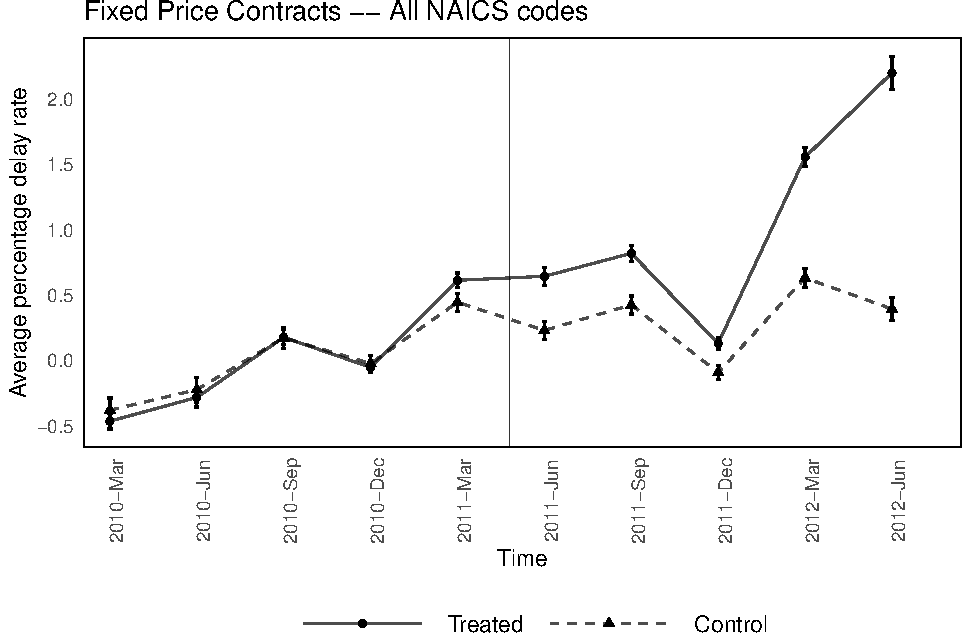
\includegraphics{o_delay_rates_main_files/figure-latex/plot_all_naics-1.pdf}

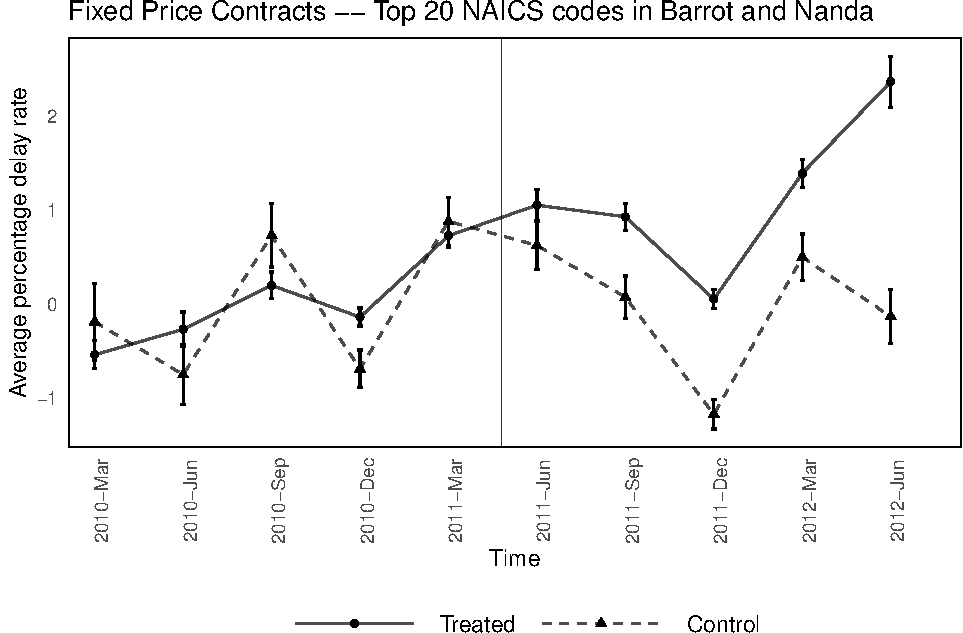
\includegraphics{o_delay_rates_main_files/figure-latex/plot_nanda_naics-1.pdf}

\end{document}
